\chapter{Related work}\label{sec:related}

    This section overviews other studies in the area of surrogate-based multi-objective optimization and related approaches of other types of optimization.


    % --------------------------------------------------------------------------------------------
    % ------------------------------------------------          Criteria
    % --------------------------------------------------------------------------------------------
    \section{Comparison criteria}
        Many existing approaches can be categorized as multi-objective optimization approaches. Therefore, the comparison criteria for a clear and concise definition of the approach are introduced in this thesis:
        \begin{description}
            \item[Sampling plan] specifies the size of a sample set from which to build a surrogate model and the sampling strategy that will pick these samples. The sampling plan can be static when decisions about samples are made ahead of time or it can be dynamic when they depend on optimization success.
            \item[Surrogate type] These criteria describe extrapolation models and a composition strategy to combine these models. In this context, variability indicates that the surrogate model is exchangeable and can be selected for a specific problem. The extensibility of a surrogate refers to the ability to grow and improve general extrapolations for a particular problem.
            \item[Optimization algorithm] is applied to find the optimal points in the search space. The architecture of the optimization algorithm and the surrogate model can be tightly coupled (\gls{osi}) either when the surrogate model is nested in the optimization algorithm, or when they perform flat architecture with alternate direct usage (\gls{aso}) \ref{fig:surr_opt_architecture}.
            \item[Scalability] Refers to the dimensionality of problems that were applied to analyze the performance of the algorithm.
            \item[Mixed search space] Parameter tuning with categorical and integer variables.
            \item[Multi-point proposal] Property of yielding the required number of multi-objective solutions.
        \end{description}

        % -------------------------------------- ASO and OSI architecture
        \begin{figure}
            \centering
            \begin{subfigure}{\textwidth}
                \centering
                \begin{subfigure}{0.45\textwidth}
                    \centering
                    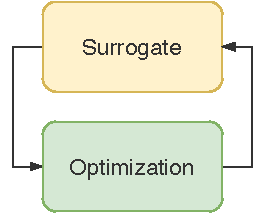
\includegraphics[height=3cm]{content/images/utility/architecture_aso}
                    \caption{Optimization with Simulation-based Iterations (OSI)}
                    \label{fig:surr_opt_architecture_aso}
                \end{subfigure} 
                \begin{subfigure}{0.45\textwidth}
                    \centering
                    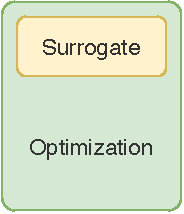
\includegraphics[height=3cm]{content/images/utility/architecture_iso}
                    \caption{Alternate Simulation-Optimization (ASO)}
                    \label{fig:surr_opt_architecture_iso}
                \end{subfigure} 
            \end{subfigure} 

            \caption[Example of a possible combination the optimization algorithm with the surrogate model.]{Example of a possible combination the optimization algorithm with the surrogate model \cite{FigueiraA14}. }
            \label{fig:surr_opt_architecture}    
        \end{figure}


        Almost all related works of parameter tuning could be categorized as \gls{smbo}\cite{JonesSW98}.
        The general \gls{smbo} looks as follows (Figure \ref{fig:sequential_mbo}):
        \begin{enumerate}
            \item Start with the initial sample plan of evaluation points.
            \item Build a regression model to provide a hypothesis about the relation between parameters and objectives.
            \item Use the built surrogate model as a parameter for optimization strategy. The solutions from the optimization algorithm are new promising points for evaluation.
            \item Evaluate the new predicted points and add them to the existing samples.
            \item If the stop criteria are not met, repeat optimization with the updated sample set.
        \end{enumerate}
        We present an overview of previous work on model-based multi-objective optimization. We begin the project for model-based optimization (mlrMBO) and continue with related algorithms including various optimization improvements.
                                                                                                    
        % ==== Sequential MBO
        \begin{figure}
            \centering 
            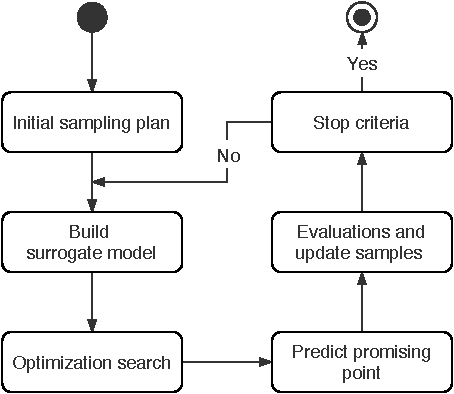
\includegraphics[width=8cm]{content/images/utility/sequential_mbo}
            \caption[General Sequential model-based optimization]{General Sequential model-based optimization (\Gls{smbo})} 
            \label{fig:sequential_mbo} 
        \end{figure}

        % Note that this approach means that

    % --------------------------------------------------------------------------------------------
    % ------------------------------------------------          Approaches
    % --------------------------------------------------------------------------------------------

    % ------------------------------------------------          Frameworks / Platforms
    \section{Platforms and frameworks}
        There are many different projects that can perform multi-objective optimization. Frameworks provide multiple multi-objective algorithms, performance metrics, built-in test problems and extra tools such as plotting and benchmarks. Some frameworks focus on efficient calculations and parallelization \cite{francesco_biscani_2019}, others on implementation of modern multi-objective algorithms \cite{benitezhidalgo2019jmetalpy, TianPlatEMO} and on support of plenty of model-based optimization algorithms \cite{BischlmlrMBO}.

        % ----------------         mlrMBO
        \paragraph{mlrMBO}\cite{BischlmlrMBO} is a modular framework for model-based optimization of expensive black-box functions. MlrBO extends the \gls{smbo} procedure to a multi-objective problem with mixed and hierarchical parameter spaces. Modular structure and integration with \emph{mlr}\footnote{{mlr}: Machine Learning in R. https://mlr.mlr-org.com/} library allows all regression models to be used and compositional techniques such as bagging and ensembling to be applied. The authors implemented four different model-based multi-objective algorithms that are categorized in three classes: 1) Scalarization-based algorithms that optimize a scalarize version of the black-box functions (\hyperref[alg:ParEGO]{ParEGO}). 2) Pareto-based algorithms that build individual models for each objective and complete multi-objective optimization (MSPOT \cite{ZaeffererBNWE13}). 3) Direct indicator-based algorithms which also fit individual models, but perform a single objective optimization on the collection of all models (SMS-EGO \cite{inproceedings}, $\epsilon$-EGO \cite{WagEGOe}).
        A special feature of the mlrMBO framework is multi-point proposal prediction on each iteration. However, it does not provide a combination of different surrogate models into one model.
       
        % ?General characteristics are that they have multiple algorithms on each type of optimization and additional features that they provide. Usually, a surrogate model is predefine and injected into some algorithm for decision making.

        % ----------------         BRISE 2.0
        \paragraph{BRISE 2.0}\label{alg:BRISE} \cite{Pukhkaiev19} is a software product line for parameter tuning. The core topics of their approach are extensibility and variability with key features such as 1) A \emph{repeater} which automatically decides on the number of repetitions needed to obtain the required accuracy for each configuration. 2) \emph{Stop condition}, which validates a solution received from the model and decides whether to stop the experiment. 3) Association of a sampling plan with model prediction validity which provides a \emph{flexible sampling plan}. The main advantage of this sampling plan is that it requires less initial knowledge about the optimization problem.
        Extrapolation model for parameter prediction is exchangeable and it combines surrogate and optimization strategies in each implementation. Several general models, such as polynomial regression surrogate with local search and Bayesian optimization with bandit-based methods strategy(BOHB \cite{FalknerBOHB}), are implemented.  However, the models lack variability and should be designed from scratch for new domain-problem.

        % ----------------         SMAC
        \paragraph{SMAC} Sequential Model-based Algorithm Configuration (SMAC)\cite{HutterHL11, smac-2017} is a framework for parameter tuning with Bayesian Optimization in combination with a simple racing mechanism to decide which of two configurations performs better.
        SMAC adopted a random forest model and Expected Improvement (EI) to model conditional probability. It applies a local search with several starting points to pick configurations with a maximal value of EI. These points improve the exploration possibilities of SMAC in the search space with higher uncertainty and an optimal value of the objective mean. 
        An interesting feature of SMAC is its support of the termination of unfavourable evaluations that are slowing down the optimization process. However, SMAC is limited to single-criteria optimization and uses a predefined sampling plan.

        % ----------------         Hypermapper
        \paragraph{Hypermapper 2.0} Luigi Nardi et al. \cite{nardi2019practical} presented a multi-objective black-box optimization framework that solves complex parameter tuning problems with the combination of search space, expensive evaluation, and feasibility constraints.
        The proposed approach can be classified as a direct indicator-based algorithm with constraint validation. During this type of optimization, several identical individual models for each objective are built, then a single-objective optimization is performed on the aggregate of all these models. The authors further extended this idea to predict no feasible configurations with an extra surrogate model.
        
        The Hypermapper 2.0 is based on a surrogate of a random forest. The random forest combines several weak regressors on a subset of samples to yield accurate regression and effective classification models. After scalarizing values from models, framework applies an Bayesian optimization (BO) method to find an optimal value. Since using a single weight vector would only find one point on the Pareto optimal front, a weight vector is chosen randomly for each iteration, ensuring that multiple points on the Pareto optimal front are found. The key features of this approach are the possibility to use prior knowledge, support real variables, predict feasibility, and excellent final adaptation of the implementation to embedded devices. The authors reported that Hypermapper 2.0 provides better Pareto fronts compared to state-of-the-art baseline, i.e. better competitive quality and saving evaluation budget.
        

    % ------------------------------------------------          Algorithms
    \section{Model-based multi-objective algorithms}
        Fixed optimization components can make general optimization ineffective in the face of different problems. The flexibility achieved by the surrogate construction methodology and multi-objective (MO) algorithms can help to achieve solutions closest to the real Pareto optimal front.

        % ----------------         ParEGO
        \paragraph{ParEGO}\label{alg:ParEGO} is a scalarization-based multi-objective algorithm \cite{Knowles06}. It was developed as extension, which can encompass multi-point proposal, of a classic single-objective algorithm \gls{ego} \cite{JonesSW98} of Jones et al. In its core lays repetition of an algorithm execution with randomly changed scalarization weights for each iteration.  This algorithm is based on the Kriging (Gaussian process regression) model and multiple single-objective optimization processes on scalarized objectives. Several runs with random weights guarantee that multiple points on the Pareto optimal front are predicted. This algorithm and its modification are implemented in mlrMBO\cite{BischlmlrMBO}.


        % ----------------         Distributed Surrogates
        \paragraph{An Evolutionary Algorithm with Spatially Distributed Surrogates} Amitay et al.,\cite{DistrSurr} presented an evolutionary algorithm with spatially distributed surrogates (EASDS). Surrogate models use Radial Basis Function Networks, periodically validating and updating each subset of samplings points. This generates a complex ensemble surrogate with approximations in local areas of the search space. Spatially Distributed Surrogate models are created for all objectives and then evaluated by NSGA-2 \cite{DistrSurr}. The authors report that their approach achieves better results than single global surrogate models, multiple surrogates. Of note, the authors evaluated their algorithm only on bi-objective problems.

        % ----------------         Hybrid surrogate
        \paragraph{A hybrid surrogate-based approach for evolutionary multi-objective optimization} Rosales-Pérez et al.,\cite{HybridSurrRCG} proposed an approach based on an ensemble of Support Vector Machines (SVM). The authors describe a model selection process or hyperparameters selection of SVM based on a validation technique and a further injection into the surrogate ensemble. Incremental development of the ensemble includes new information obtained during the optimization and old evidence stored in previous models. 
        The training of a new model represents search on the SVM grid in order to find a kernel with the lowest expected generalization error. This paper presents a model selection process for determining the hyperparameters for each SVM in the ensemble.


        % ----------------         Hierarchical surrogates
        \paragraph{Evolutionary optimization with hierarchical surrogates} Xiaofen Lu et al. \cite{LuST19} apply different surrogate modelling techniques based on the motivation to optimize expensive black-box functions without any prior knowledge of the problem. They used a pre-specified set of models to construct hierarchical surrogates during optimization. Also, to verify the surrogates, the general accuracy of the high-level model was used. The process of the proposed method involves splitting the accumulated training samples and model-based optimization, which means that the sample plan is static and requires prior information about the problem. 

        The authors show that the hierarchical surrogate structure can be beneficial when the accuracy of the high-level model is greater than 0.5. They also noticed that a single modelling technique might perform differently on different problem landscapes. This motivates us to use a pre-specified set of modelling techniques (portfolio with surrogates).
        
        % ----------------         Local search in parallel surrogates 
        \paragraph{Population-based Parallel Surrogate Search} Akhtar et al.,\cite{akhtar2019efficient} introduce a multi-objective optimization algorithm for expensive functions that connects several iteratively updated surrogates of the objective functions. The key feature of this algorithm is high optimization for parallel computation and stacking predictions from the set of Radial Basis Function (RBF) models. The algorithm combines RBF composition surrogate, Tabu, and local search around multiple points. 
        % The authors present an algorithm that can theoretically be applicable to high-dimensional spaces and many-objective problems because the selected surrogate and optimization algorithm are well scalable.


        % ----------------         GALE
        \paragraph{GALE: Geometric Active Learning for Search-Based Software Engineering} Krall et al.,\cite{KrallMD15} developed an algorithm that uses principal components analysis (PCA) and active learning techniques to perform step-by-step approximation and evaluation of the most informative solutions. The authors notice that MOEAs are not suitable for expensive multi-objective problems because they push a set of solutions towards an outer surface of better candidates, costing many function evaluations. The fundamental idea of the proposed approach is to choose the most informative solutions from a large set of options. This is accomplished by dividing the functional landscape into smaller regions and evaluating only the most informative samples from the regions. As a result of the division of the functional landscape, function evaluations are spared since only a few of the most informative points from the region are evaluated. A drawback of this approach lays in static implementation with MOEA/D.        


        % ===== TABLE
    \begin{table}[]
        \centering
        \caption{The comparison of related approaches. The component behaviour: S - static, V - variability, E-extensibility, D - dynamic}
        \label{tab:my-table}
        \resizebox{\textwidth}{!}{%
        \begin{tabular}{@{}|l|c|c|c|c|c|c|c|c|@{}}
        \toprule
        \multicolumn{1}{|c|}{\multirow{2}{*}{Approach}} &
        \multirow{2}{*}{Multi-objective} &
        \multirow{2}{*}{Sampling plan} &
        \multicolumn{2}{c|}{Surrogate} &
        \multirow{2}{*}{Optimization} &
        \multirow{2}{*}{\begin{tabular}[c]{@{}c@{}}Mixed \\ search space\end{tabular}} &
        \multirow{2}{*}{\begin{tabular}[c]{@{}c@{}}Multi-point \\ proposal\end{tabular}} &
        \multirow{2}{*}{Scalability} \\ \cmidrule(lr){4-5}
        \multicolumn{1}{|c|}{} &
        &
        &
        \begin{tabular}[c]{@{}c@{}}Extrapolation \\ models\end{tabular} &
        \begin{tabular}[c]{@{}c@{}}Composition \\ strategy\end{tabular} &
        &
        &
        &
        \\ \midrule
        mlrMBO\cite{BischlmlrMBO} &
        \cmark &
        static &
        E &
        \multicolumn{2}{c|}{V} &
        \cmark &
        \cmark &
        \cmark \\ \midrule
        BRISE 2.0 \cite{Pukhkaiev19} &
        \xmark &
        flexible &
        \multicolumn{3}{c|}{V} &
        \cmark &
        \cmark &
        \cmark \\ \midrule
        SMAC \cite{HutterHL11}&
        \xmark &
        static &
        S &
        S &
        S &
        \cmark &
        \xmark &
        \cmark \\ \midrule
        Hypermapper 2.0 \cite{nardi2019practical} &
        \cmark &
        flexible &
        S &
        S &
        S &
        \cmark &
        \xmark &
        \cmark \\ \midrule
        ParEGO \cite{Knowles06} &
        \cmark &
        static &
        S &
        S &
        S &
        \xmark &
        \xmark &
        \cmark \\ \midrule
        \begin{tabular}[c]{@{}l@{}}Distributed Surrogates, \\ EASDS \cite{DistrSurr}\end{tabular} &
        \cmark &
        static &
        S &
        E &
        S &
        \xmark &
        possible &
        \xmark \\ \midrule
        Hybrid surrogate \cite{HybridSurrRCG} &
        \cmark &
        static &
        S &
        E+D &
        V &
        \xmark &
        possible &
        \cmark \\ \midrule
        Hierarchical surrogates \cite{LuST19}&
        \xmark &
        static &
        E &
        V &
        V &
        \xmark &
        possible &
        \xmark \\ \midrule
        \begin{tabular}[c]{@{}l@{}}Parallel surrogates, \\ MOPLS \cite{akhtar2019efficient}\end{tabular} &
        \cmark &
        static &
        S &
        E &
        S &
        \xmark &
        \cmark &
        \xmark \\ \midrule
        GALE \cite{KrallMD15}&
        \cmark &
        static &
        S &
        E &
        S &
        \cmark &
        possible &
        \cmark \\ \bottomrule
        \end{tabular}%
        }
        \end{table}

    % --------------------------------------------------------------------------------------------
    % ------------------------------------------------          Conclusions
    % --------------------------------------------------------------------------------------------
    \section{Scope of work}

        As shown before, surrogate or model-based optimization suit expensive black-box problems. A summary of the related works that we have discussed is shown in Table \ref{tab:my-table}. Nevertheless, model-based approach still has limitations:
        \begin{itemize}
            \item Multi-objective hypothesis. A \emph{limited number} of surrogate models can handle with several parameter and objectives, but they struggle when these parameters and objectives become larger. 
            \item \emph{Surrogate is domain-specific.} Currently, to improve and reach the best prediction, we need to know the objective surface in order to apply a specific surrogate. Universal surrogates might gain optimal results but may not be the most reliable \cite{abs181207958, LuST19}. 
            \item The quality of predictions depends on \emph{the number of samples} we use for a specific type of surrogate. There is a trade-off between the reduction of sample size and maximization of prediction quality. Overfitting, as well as underfitting, can guide optimization in a wrong direction.
            \item Often, optimization algorithms and surrogate models are \emph{coupled} extremely tightly. This interdependence makes the general approach biased against specific problems. Reimplementation of these algorithms for each usage scenario becomes time-consuming and error-prone.
        \end{itemize}

        After surveying the aforementioned literature, we derive the following research gaps and questions:
        \begin{description}
            \item[Surogate combination] Previous research has shown that surrogate model selection can profoundly impact the quality of the optimization solution \cite{HybridSurrRCG}. Furthermore, it has been noted that the surrogate is domain-specific, and the same technique might perform differently on different problems \cite{LuST19}. The overall research gaps of the surrogate model's flexibility can be divided into the following subproblems:
            \begin{enumerate}
                \item The dynamic combination of different single-criterion models is crucial to solve the multi-criteria problems. It must be feasible to substitute the type of nested surrogate model for an arbitrary criterion component. This would make the suggorate model more versatile and capable of describing arbitrary optimization problems. Therefore, technology that would allow the creation of surrogate compositional models is necessary. Hence we can identify the first research question \textbf{[RQ1]}: How to dynamically combine different single-objective models to extrapolate multi-objective problems?
                \item After scrupulous investigation of presented works we conclude that access to the range of models improves final results. Unfortunately, most authors used only one type of model with various hyperparameters. Therefore, the next research question \textbf{[RQ2}]: How to combine surrogate models in a portfolio?
            \end{enumerate}
            \item[Sampling plan] A static plan requires additional knowledge of the surface of the problem, which is usually not possible to obtain. Moreover, arbitrary decisions of the sample size might be a reason that leads to inaccurate models and further wrong results. These problems may occur because the surrogate model is overfitted or underfitted, and the result is a waste of samples and resources. Consequently, the last research question \textbf{[RQ3]}: How to select an appropriate sampling plan?
        \end{description}

        To our knowledge, there have not been studies of the comprehensive surrogate combinations and the dynamic sampling strategy.   Therefore, we focus on the improvement of compositional surrogate models for multi-objective problems. We aim to apply surrogate models to problems that are expensive, multi-objective, and derivative-free/black-box systems without constraints.
        \paragraph{The following goals must be achieved:}
        \begin{enumerate}
            \item Find diverse multi-objective solutions with minimal distance to real the Pareto front. 
            \item Develop modular and extensible architecture. 
            \item Improve the backward computationally with single-objective parameter tuning.
            \item Reduce the evaluation budget.
        \end{enumerate}






        % In this thesis, we focus on the improvement of surrogate models for multi-objective problems. Surrogate-based optimization has proven its effectiveness in many areas of engineering and in applications where data is expensive or difficult to evaluate. While other methods also exist, we select \gls{moea} as the main solver because it can be applied to a wide range of problems and because it gives a broad understanding of how the Pareto front looks.  % many areas of engineering --- CARL where are references/proofs ? or remove many and in before applications






        % Also optimization and composition of multi-objective solvers is a rapidly expanding area of research and a full survey of that work is beyond the scope of this thesis.



        % --------------------------------------------------------------------------
        % Fixed components can make the optimization of changeable problems ineffective. 
        % Appropriate surrogate construction methodology or combination of multiple solving algorithms could improve the final solution. The significant works analyze that compositional architecture with several surrogate models is a promising direction to improve the multi-objective solution. 
        % Moreover, almost none of the approaches examined the size of the surrogate sample set. 

        % !There is a clear need for a method to provide and distribute ready-to-use implementations of optimization methods and ready-to-use benchmark and real-world problems. These modules should be freely combinable. Since the above mentioned issues are not constrained to evolutionary optimization a candidate surrogates solution should be applicable to a broader range of search algorithms



        % However, it lacks fundamental features that makes it ineffective in the presence of applications with non-feasible designs and prior knowledge.


        % Our work is similar in nature to the approaches adopted in the Bayesian optimization literature [27]. Example of widely used mono-objective Bayesian DFO software are SMAC [15], SpearMint [30], [31] and the work on tree-structured Parzen estimator (TPE) [6]. In particular, the use of a full Bayesian ap- proach will help to leverage the prior knowledge by computing a posterior distribution. Exploration of additional methods to warm-up the search from the design of experiments literature

        % \paragraph{Hyperopt}




        % Based on a survey\cite{SoftSurvey} there still exist such as:
        % \begin{itemize}
        %     \item 
        % \end{itemize}


        % Some features of their approach are 


        % We extend the idea of stochastic RBF to be suitable for the algorithm configuration task. It is a model-based algorithm that cycles from emphasis on the objective to emphasis on the distance using a weighting strategy. 
        
        % The main advantage of LHS is that it does not require an increased initial population size for more dimensions.


        % exploration, exploitation and diversification during each algorithm iteration.


        % To our knowledge, there exists no research that investigates how deep networks affect the performance of surrogate-assisted multi-objective evolutionary algorithms. If neural networks were used, the approaches usually adopted only one hidden layer. Additionally, we can also see that there exists a multitude of ways a surrogate model can be integrated into an evolutionary algorithm

        % Previous studies have shown that the choice of modeling technique can highly affect the performance of the surrogate model-assisted evolutionary search.

        % However, one modeling technique might perform differently on different problem landscapes. Without


        % OpenTuner is different from our work in a number of ways. First, our work supports multi-objective optimization. Second, our white-box model-based approach enables the user to understand the results while learning from them. Third, our approach is able to consider unknown feasibility constraints. Lastly, our framework has the ability to inject prior knowledge into the search. The first point in particular does not allow a direct performance comparison of the two tools.

        % over the entire space would result in a waste of samples.


        % This is especially the case for a SMBO

        % The black-box function can be more complex, for example a machine learning pipeline which includes preprocessing, feature selection and model selection.


        % Consequently, the advantage of the multi-objective candidate generation to produce a set instead of single points is not only used for improving the exploration of the decision space, but also for obtaining a well-spread batch of solutions.


        % For example, OEGADO \cite{ChafekarSRX05} creates a surrogate model for each of the objectives. The best solutions in every objective get also approximated on other objectives, which helps with finding trade-off individuals. The best individuals are then exactly evaluated and used to update the models.


        % ? Bayesian optimization (BO) methods often rely on the assumption that the objective function is well-behaved, but in practice, the objective functions are seldom well-behaved even if noise-free observations can be collected. In \cite{bodin2019modulating} propose robust surrogate models to address the issue by focusing on the well-behaved structure informative for search while ignoring detrimental structure that is challenging to model data efficiently.